%%%%%%%%%%%%%%%%%%%%%%%%%%%%%%%%%%%%%%%%
%%%%% PRIOR RESEARCH
%%%%%%%%%%%%%%%%%%%%%%%%%%%%%%%%%%%%%%%%
\section{PRIOR RESEARCH}
    \subsection{Prior Music Recommendation}
        \subsubsection{Deep Content-Based Music Recommendation \cite{NIPS2013_5004}}
        
        The Deep Content-Based Music Recommendation paper proposed a very unique approach to address problems with the current music recommender systems. In this paper, they have attempted to analyze a latent factor vectors, which is a compact description of user\'s tastes and corresponding characteristics of items, based on the preference in past. Because the music audio signal is used to characterized music, this approach is less likely to result in an unfair result for unpopular artists. They have tested two approaches to predict latent factors, a method using Bag of Words representation on Mel-frequency Cepstrum Coefficients and a method using Convolutional Neural Networks.
        
        \subsubsection{Improving Content-based and Hybrid Music Recommendation Using Deep Learning \cite{Wang:2014:ICH:2647868.2654940}}
        
        Music recommender system with traditional content based music analysis, which uses high level property of music such as Mel-frequency Cepstral Coefficients, often has unsatisfactory result in accuracy. This paper utilized a novel model and probabilistic graphical model to recommend songs by using both collaborative filtering of metadata as well as analysis on learned feature from audio content. Their Hierarchical linear model with a deep belief network particularly improves the accuracy of prediction in a warm start stage. 
        
        \subsubsection{Collaborative Deep Learning for Recommender Systems \cite{Wang2014}}
        In this paper, a method called Collaborative Deep Learning was proposed to address the problem with information insufficiency. With music recommendation systems using Collaborative Filtering, the accuracy drops significantly when the ratings given by users are insufficient. On the other hand, when recommending music using latent representations, the result may not be very effective if the auxiliary information is insufficient. While a statistical model, Collaborative topic regression, can be used to bridge collaborative filtering methods and latent representation methods, lack of sufficient information can still degrade the accuracy of recommendations. However, this new method, collaborative deep learning, solves this problem by jointly performing deep learning for the content information and collaborative filtering for the ratings by using hierarchical Bayesian models.

    \subsection{LSTM \cite{Hochreiter1997}}
        \begin{figure}[H]
            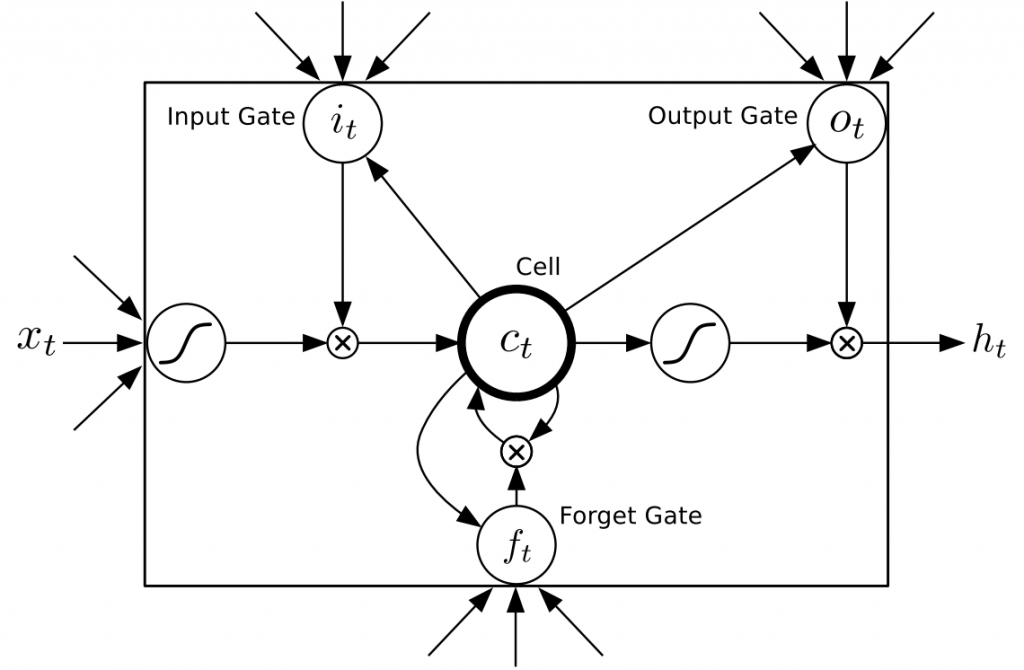
\includegraphics[width=0.45\textwidth]{lstm_cell.png}
            \caption{LSTM Cell Representation}
            \label{fig:lstm-cell}
        \end{figure}
        LSTM is a type of Recurrent Neural Network, specializing to work with long term dependencies. Typically, an LSTM network is composed of cells (depicted in figure \ref{fig:lstm-cell}) containing an input gate, output gate, forget gate, and at least one memory cell. The input gate controls what value can be entered into the memory cell, the output gate controls which of the values in the cell should be used, and forget gate controls which value in the cell should remain. By having such an architecture, a neural network utilizing the LSTM framework excels at understanding input information using what it has learned before, making it an ideal framework for audio analysis. The recent success in using Neural Networks for tasks such as speech recognition is due to this framework.